%
%===============>>  ПРОБНИК 1 <<=============
%

%BEGIN_FOLD % ====>>_____ Вариант 1 _____<<====
\begin{training}[1]
	\title{Часть 1}
	\begin{listofex}
		%1
		\item Для объектов, указанных в таблице, определите, какими цифрами они обозначены на схеме. Заполните таблицу, в ответ запишите последовательность четырёх цифр.
			\begin{center}
			\footnotesize
			\begin{tabular}{|g|c|c|c|c|}
				\hline
				\textbf{Объекты}&Туалет&Детская&Гостиная&Кухня\\
				\hline
				\textbf{Цифры}&&&&\\
				\hline
			\end{tabular}
		\end{center}
			На плане изображена схема квартиры (сторона каждой клетки на схеме равна \( 1 \) м). Вход и выход осуществляются через единственную дверь.
		\gapwidth
		\begin{center}
			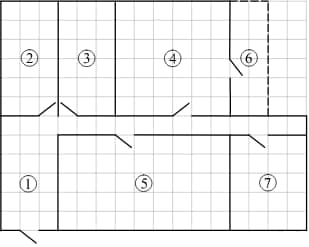
\includegraphics[align=t, width=0.5\linewidth]{\picpath/prob_2.2_1}
		\end{center}
		%2
		\item Краска продаётся в банках по \( 3 \) л. Сколько банок краски требуется купить, чтобы покрасить потолок в гостиной?
			\foranswer
		%3
		\item Найдите площадь, которую занимают детская и балкон. Ответ дайте в квадратных метрах.
		\foranswer
		%4
		\item Найдите расстояние между противоположными углами детской комнаты в метрах. Ответ запишите в виде \( \dfrac{d}{\sqrt{2}} \).
	\end{listofex}
	\newpage
	\phantom{Часть 1}
	\begin{listofex}[resume]
		%5
		\item 
			Хозяин квартиры планирует установить в квартире счётчик. Он рассматривает два варианта: однотарифный или двухтарифный счётчики. Цены на оборудование и стоимость его установки, данные о потребляемой мощности, и тарифах оплаты даны в таблице.
			Обдумав оба варианта, хозяин решил установить двухтарифный электросчётчик. Через сколько дней непрерывного использования электричества экономия от использования двухтарифного счётчика вместо однотарифного компенсирует разность в стоимости установки двухтарифного счётчика и однотарифного?
			\foranswer
		\gapwidth
		\begin{center}
			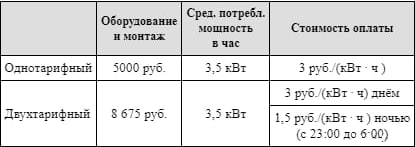
\includegraphics[align=t, width=0.8\linewidth]{\picpath/prob_2.2_2}
		\end{center}
		%6
		\item Найдите значение выражения \( \cos\dfrac{5\pi}{6}\cdot\tg\dfrac{4\pi}{3} \)
		\foranswer
		%7
		\item
		На рисунке изображён график функции \( y=f(x) \) и касательная к нему в точке с абсциссой \( x_0 \). Найдите значение производной функции \( f(x) \) в точке \( x_0 \).
		\begin{center}
			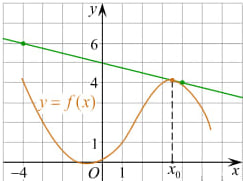
\includegraphics[align=t, width=0.5\linewidth]{\picpath/prob_2_4}
		\end{center}
		\foranswer
		%8
		\item К источнику с ЭДС \( \epsilon=55 \) В и внутренним сопротивлением \( r=0,5 \) Ом, хотят подключить нагрузку с сопротивлением \( R \) Ом. Напряжение на этой нагрузке, выражаемое в вольтах, даeтся формулой \( U=\dfrac{\epsilon R}{R+r} \).  При каком наименьшем значении сопротивления нагрузки напряжение на ней будет не менее \( 50 \) В? Ответ выразите в омах.
		\foranswer
		%9
		\item Первая труба пропускает на \( 3 \) литра воды в минуту меньше,
		чем вторая. Сколько литров воды в минуту пропускает вторая труба,
		если резервуар объемом \( 594 \) литра она заполняет на \( 5 \) минут быстрее,
		чем первая труба заполняет резервуар объемом \( 648 \) литров?
		\foranswer
		\newpage
		\hphantom{Часть 1}
		%10
		\item 
		На рисунке изображены графики функций \( f(x) = a\sqrt{x-b}+c \) и \( g(x) = 0,75x+1 \),
		которые пересекаются в точках \( A(0;1) \) и \( B \). Найдите абсциссу точки \( B \).
		\begin{center}
			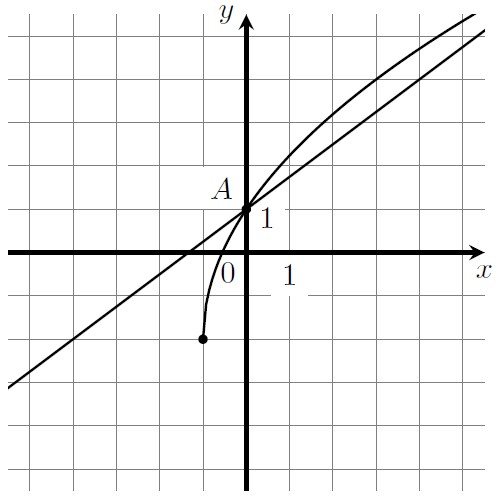
\includegraphics[align=t, width=0.4\linewidth]{\picpath/prob_1_10}
		\end{center}
		\foranswer
		%11
		\item Найдите наименьшее значение функции \( y=-x^3-27+75x \) на отрезке \( [-5;5] \).
		\foranswer
		%12
		\item .
		%13
		\item .
		%14
		\item .
		%15
		\item .
		%16
		\item .
		%17
		\item .
		%18
		\item .
		%19
		\item .
		\title{Часть 2}
		%20
		\item .
		%21
		\item .
		%22
		\item .
		%23
		\item .
		%24
		\item .
		%25
		\item .
	\end{listofex}
\end{training}
%END_FOLD

%BEGIN_FOLD % ====>>_____ Вариант 2 _____<<====
\begin{training}[2]
	\title{Часть 1}
	\begin{listofex}
		%1
		\item
		Длина зонта в сложенном виде равна \( 27 \) см и складывается из длины ручки (рис. \( 3 \)) и трети длины спицы (зонт в три сложения). Найдите длину спицы, если длина ручки зонта равна \( 6,8 \) см.\\\\
		Две подруги Оля и Аня задумались о том, как рассчитать площадь поверхности зонта.\\
		На первый взгляд зонт кажется круглым, а его купол напоминает часть сферы (сферический сегмент). Но если присмотреться, то видно, что купол зонта состоит из двенадцати отдельных клиньев, натянутых на каркас из двенадцати спиц (рис. \( 1 \)). Сферическая форма в раскрытом состоянии достигается за счёт гибкости спиц и эластичности ткани, из которой изготовлен зонт.\\
		Оля и Аня сумели измерить расстояние между концами соседних спиц \( a \). Оно оказалось равно \( 28 \) см. Высота купола зонта \( h \) (рис. \( 2 \)) оказалась равна \( 27 \) см, а расстояние \( d \) между концами спиц, образующих дугу окружности, проходящей через вершину зонта, --- ровно \( 108 \) см.
			\foranswer
		\gapwidth
		\begin{center}
			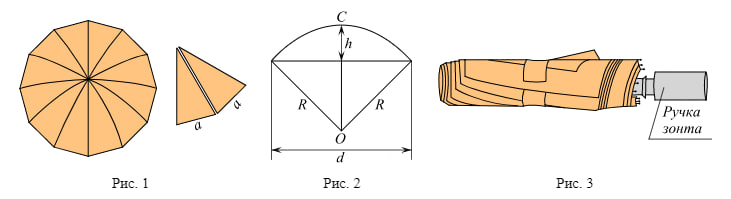
\includegraphics[align=t, width=\linewidth]{\picpath/prob_2.2_3}
		\end{center}
		\foranswer
		%2
		\item
		Поскольку зонт сшит из треугольников, рассуждала Оля, площадь его поверхности можно найти как сумму площадей треугольников. Вычислите площадь поверхности зонта методом Оли, если высота каждого равнобедренного треугольника, проведённая к основанию, равна \( 59 \) см. Ответ дайте в квадратных сантиметрах с округлением до десятков.
		\foranswer
		
		\newpage
		\hphantom{Часть 1}
		%3
		\item Аня предположила, что купол зонта имеет форму сферического сегмента. Вычислите радиус \( R \) сферы купола, зная, что \( OC=R \) (рис. \( 2 \)). Ответ дайте в сантиметрах.
		\foranswer
		%4
		\item Аня нашла площадь купола зонта как площадь поверхности сферического сегмента по формуле \( S=2\pi Rh \), где \( R \) --- радиус сферы, a \( h \) --- высота сегмента. Рассчитайте площадь поверхности купола способом Ани. Число \( \pi \)  округлите до \( 3,14 \). Ответ дайте в квадратных сантиметрах с округлением до целого.
		\foranswer
		%5
		\item Рулон ткани имеет длину \( 20 \) м и ширину \( 90 \) см. На фабрике из этого рулона были вырезаны треугольные клинья для \( 15 \) зонтов, таких же, как зонт, который был у Оли и Ани. Каждый треугольник с учётом припуска на швы имеет площадь \( 850 \) кв. см. Оставшаяся ткань пошла в обрезки. Сколько процентов ткани рулона пошло в обрезки?
		\foranswer
		%6
		\item Найдите \( 20\cos2x \), если \( \cos x = 0,1 \)
		\foranswer
		%7
		\item 
		Материальная точка движется прямолинейно по закону \( x(t)=\dfrac{1}{6}t^2+5t+28 \) (где \( x \)  --- расстояние от точки отсчета в метрах, \( t \) --- время в секундах, измеренное с начала движения). В какой момент времени (в секундах) ее скорость была равна \( 6 \) м/с?
		\foranswer
		%8
		\item В ходе распада радиоактивного изотопа его масса уменьшается по закону \( m(t)=m_0\cdot2^{-t/T} \), где \( m_0 \) --- начальная масса изотопа, \( t \) --- время, прошедшее от начального момента, \( T \) --- период полураспада. В начальный момент времени масса изотопа \( 188 \) мг. Период его полураспада составляет \( 3 \) мин. Найдите, через сколько минут масса изотопа будет равна \( 47 \) мг.
		\foranswer
		\newpage
		\hphantom{Часть 1}
		%9
		\item Первый и второй насосы наполняют бассейн за \( 9 \) минут,
		второй и третий --- за \( 12 \) минут, а первый и третий --- за \( 18 \) минут.
		За сколько минут эти три насоса заполнят бассейн, работая вместе?
		\foranswer
		%10
		\item 
		На рисунке изображены графики функций \( f(x) = \frac{k}{x} \) и \( g(x) = ax+b \),
		которые пересекаются в точках \( A(-2;-3) \) и \( B \). Найдите абсциссу точки \( B \).
		\begin{center}
			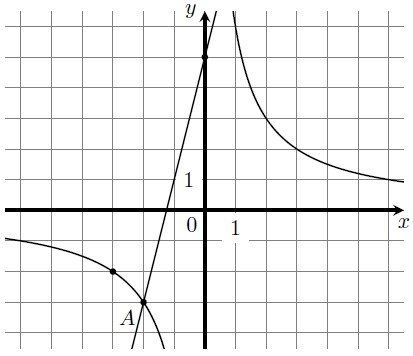
\includegraphics[align=t, width=0.4\linewidth]{\picpath/prob_1_8}
		\end{center}
		\foranswer
		%11
		\item Найдите наименьшее значение функции \( y=13+75x-x^3 \) на отрезке \( [-5;5] \).
		\foranswer
		%12
		\item .
		%13
		\item Ю
		%14
		\item .
		%15
		\item .
		%16
		\item .
		%17
		\item .
		%18
		\item .
		%19
		\item .
		\title{Часть 2}
		%20
		\item .
		%21
		\item .
		%22
		\item .
		%23
		\item .
		%24
		\item .
		%25
		\item .
	\end{listofex}
\end{training}
%END_FOLD